\chapter{Computational implementation of quantum and classical hierarchical equations of motion}
\chaptermark{Computational implementation of HEOM}
Quantum hierarchical equations of motion (HEOM) were implemented and tested in their reduced high-temperature form, where Matsubara terms from the bath time autocorrelation function are omitted. This is presented in section \ref{sec:qheom}. Classical HEOM in position-momentum phase space are studied in section \ref{sec:cheom}. Following the low-temperature breakdown of the previous implementation of quantum HEOM, their full form including the Matsubara terms was investigated in section \ref{sec:qheom_low_temp}. Two anharmonic potentials were studied using the implemented methods: a Morse oscillator in section \ref{subsec:morse} and a fitted OH potential of a hydrated oxonium ion in section \ref{subsec:anharmonic}.
\clearpage
%\newpage
\section{High-temperature quantum HEOM}\label{sec:qheom}
Taking the work of Tanimura and Wolynes as inspiration,\supercite{Tanimura1991a} the high-temperature quantum HEOM described by eq.~\ref{eq:qheom_high_temp} were implemented.

The density matrix was represented in the basis of position eigenvectors $q_i \equiv \delta(q-q_i)$. The position operator and the potential energy operator are diagonal in this representation, giving
\begin{equation}
\begin{split}
\frac{\partial \rho_{n}(q_i,q_j) }{\partial t} =
&-\left(\frac{\mathrm{i}}{\hbar}\hat{\mathcal{L}}+n \gamma \right)\rho_{n}(q_i,q_j)
-\frac{\mathrm{i}}{\hbar}(q_i - q_j) \rho_{n+1}(q_i,q_j) \\
&-\frac{n_0 \eta\gamma^2}{2}(q_i + q_j) \rho_{n-1}(q_i,q_j) \\
&-\frac{\mathrm{i}}{\hbar}\frac{n \hbar \eta \gamma^2}{2}\cot\left(\frac{\beta\hbar\gamma}{2}\right)(q_i - q_j) \rho_{n-1}(q_i,q_j).
\end{split}
\end{equation}
To express the Hamiltonian in this basis, a discrete variable representation (DVR) matrix for the second derivative (the momentum operator) was used to obtain\supercite{Colbert1992}
\begin{equation}
	H_\mathrm{S}(q_i,q_j) =
	 \begin{cases}
	 V(q_i) +\frac{\hbar^2\pi^2}{6 m (\Delta q)^2}& \text{for }i=j, \\
	 \frac{\hbar^2 }{m (\Delta q)^2 (i-j)^2}(-1)^{i-j} & \text{otherwise,}
	 \end{cases}
	 \label{eq:dvr_ham}
\end{equation}
where $\Delta q\equiv q_{i+1}-q_i$ is the position grid spacing. The equations of motion were then integrated in time using the fourth-order Runge-Kutta method.\supercite{Press1992, Press1996}

The general behaviour was investigated in a shifting harmonic potential as described in section~\ref{subsec:qheom_shifting_potential} and position time autocorrelation functions were calculated (TCFs) in section~\ref{subsec:qheom_tcfs}. As expected, these simulations deteriorated with decreasing temperature, when the truncation of the bath-coordinate time autocorrelation function $\alpha$ (eq.~\ref{eq:alpha_series}) gives an increasingly large error.

\subsection{Shifting potential}\label{subsec:qheom_shifting_potential}
To test this set-up, we implemented the system presented in Tanimura's original paper,\supercite{Tanimura1991a} which is a harmonic oscillator with a variable linear term given by
\begin{equation}
	V_\mathrm{S}(q) = \frac{m \Omega^2}{2}q^2 - Fq,
\end{equation}
where
\begin{equation}
	F =
	\begin{cases}
	0 & \text{for }t<0 \\
	6 & \text{for }t\ge 0
	\end{cases},
\end{equation}
$\Omega=2$ and $m=1$, all in atomic units. The initial state in the simulation was the Boltzmann distribution for the isolated system, which is given by
\begin{multline}
	\rho_0 (q_i,q_j) = \sqrt{\frac{m\Omega}{2\pi \hbar \sinh(\beta\hbar\Omega)}}\\
	\times\exp\left[-\frac{m\Omega}{2\pi \hbar \sinh(\beta\hbar\Omega)} \left[(q_i^2+q_j^2)\cosh(\beta\hbar\Omega)-2 q_i q_j\right]\right]
	\label{eq:ho_init_state}
\end{multline}
with all ADOs set to zero (i.e.~the factorised initial condition of eq.~\ref{eq:factorised}).

The system was allowed to equilibrate and then the potential was shifted, which resulted in damped oscillations. This behaviour is shown in fig.~\ref{fig:qheom_contour}. The rate of the damping is affected both by the bath strength $\eta$ and by the cutoff frequency $\gamma$, which is illustrated in figure~\ref{fig:qheom_position}. Both of these trends follow the expected behaviour. Increasing the strength of the bath coupling leads to higher damping and so does increasing the cutoff frequency.

\begin{figure} [hb!] %pro lepsi obplouvani textu
	\centering
	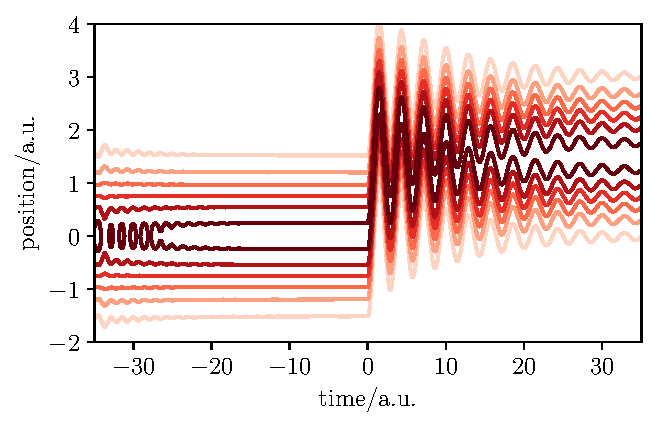
\includegraphics [width=11cm]{qheom_contour.pdf}
	\caption{
		A contour plot of a wavepacket being equilibrated with a bath in a harmonic potential centered at $q=0$. At $t=0$ the potential is shifted by an addition of a linear term, which creates a new minimum at $q=3/2$~a.u. This is a reproduction of a similar calculation from Tanimura, Wolynes, \emph{Phys.~Rev.~A}, 1991, \textbf{43}, 4131–4142.
	}
	\label{fig:qheom_contour}
\end{figure}
\begin{figure} [htp!] %pro lepsi obplouvani textu
	\centering
	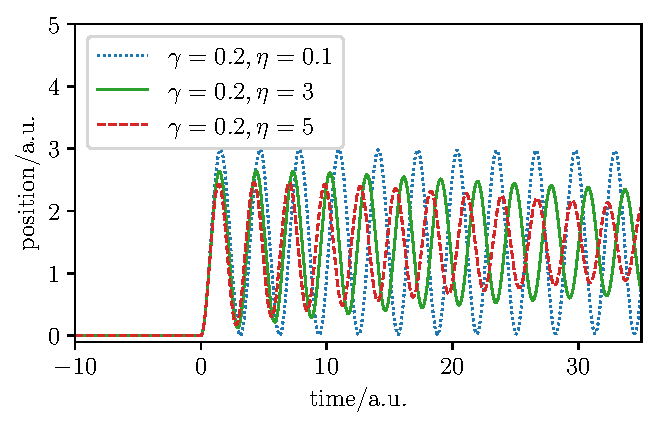
\includegraphics [width=11cm]{qheom_position_eta.pdf}
	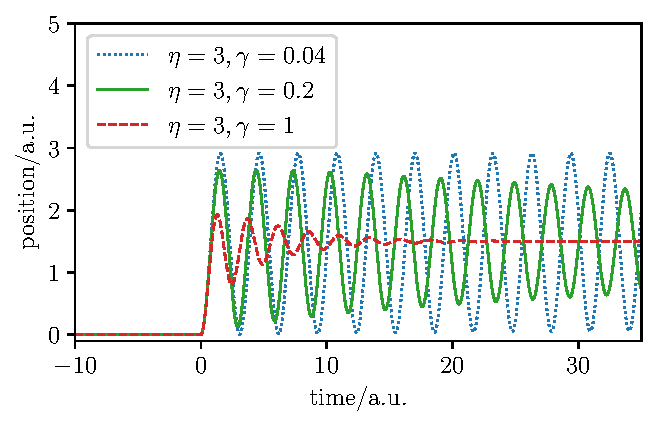
\includegraphics [width=11cm]{qheom_position_gamma.pdf}
	\caption{
		Displacement of the wavepacket centre (average) for a set-up described in fig.~\ref{fig:qheom_contour} as a function of the bath strength $\eta$ and the bath cutoff frequency $\gamma$.
	}
	\label{fig:qheom_position}
\end{figure}

\clearpage
\subsection{Harmonic potential TCFs}\label{subsec:qheom_tcfs}
Dynamical properties of quantum systems are often described using time correlation functions (TCFs). These can then be used to predict vibrational spectra, diffusion coefficients, reaction rates and many other experimental observables.\supercite{Zwanzig2001,Nitzan2013} We have chosen the position time autocorrelation function as a good means of probing the system, because it is closely related to the infra-red vibrational spectrum. The TCF is defined as
\begin{multline}
	C_{qq} (t)
	= \langle \hat{q}(\tau)\hat{q}(\tau+t)\rangle
	= \langle \hat{q}(0)\hat{q}(t)\rangle = \\
	= \mathrm{Tr}\left[\hat{\rho}\hat{q}(0)\hat{q}(t)\right]
	= \mathrm{Tr}\left[\hat{\rho}\hat{q}\mathrm{e}^{+\mathrm{i}\hat{H}t/\hbar}\hat{q}\mathrm{e}^{-\mathrm{i}\hat{H}t/\hbar}\right],
	\label{eq:tcf_qq}
\end{multline}
where we have used the fact that for an equilibrium state TCFs are independent of the time origin.\footnote[2]{This is due to the commutation of the time evolution and Boltzmann density operator for time independent Hamiltonians.} The last expression can be evaluated by propagating the density matrix $\hat{\rho}\hat{q}$ in time using the HEOM and then acting on it by $\hat{q}$ and summing the trace for each sampled time.
%\footnote[3]{Strictly speaking, we obtain the complex conjugate of the TCF, because we are calculating $\mathrm{Tr}\left[(\hat{\rho}\hat{q})(t)\hat{q}(0)\right] = C_{qq}(-t) = C_{qq}^*(t)$.\supercite{Nitzan2013}}

A useful way of presenting TCFs is by taking their Fourier transform, which is also called the power spectrum, and is given by
\begin{equation}
	G_{qq}(\omega) = \int_{-\infty}^{\infty}\mathrm{d}t\ \mathrm{e}^{\mathrm{i}\omega t}C_{qq}(t).
\end{equation}
Assuming that the dipole moment is proportional to the displacement of our system, and employing Fermi's golden rule, the power spectrum can be related to the  vibrational absorption spectrum as\supercite{Zwanzig2001}
\begin{equation}
	I(\omega) \propto \omega (1-\mathrm{e}^{-\beta\hbar\omega})G_{qq}(\omega),
\end{equation}
where the frequency-independent constant of proportionality depends the on physical parameters of the measurement. All spectra in this work are presented in arbitrary units.

In the TCF of the harmonic oscillator system described in the previous section we can clearly see the damping effect of the ``random force" of the bath, which leads to a loss of coherence and decorrelation as shown in figure~\ref{fig:qheom_tcf_gamma}. Increasing the cutoff frequency of the bath $\gamma$ leads to shorter decorrelation times. This can also be observed in the spectrum as broadening and shifting of the peak. It should be noted that the blue shift is due to the renormalisation potential of eq.~\ref{eq:renorm_pot}, rather than the dynamics of the bath.
\newpage
When the temperature is sufficiently low ($\beta\hbar\Omega\gg1$), we observe non-physical ``beats" which are an artefact of the truncation of the bath-coordinate time autocorrelation function $\alpha$ (eq.~\ref{eq:alpha_series}). At very low temperatures the TCF simply diverges without ever being damped to zero. In addition, during equilibration at low temperatures, the wave packets have a tendency to dissolve, grow rapidly, change shape or drift, all of which make simulations less stable as well as non-physical. This is illustrated in figure~\ref{fig:qheom_tcf_beta} where the TCF becomes well behaved only for very short times with increasing $\beta$. Similar behaviour was observed for anharmonic potentials in sections \ref{subsec:morse} and \ref{subsec:anharmonic}.

\begin{figure} [htp!] %pro lepsi obplouvani textu
	\centering
	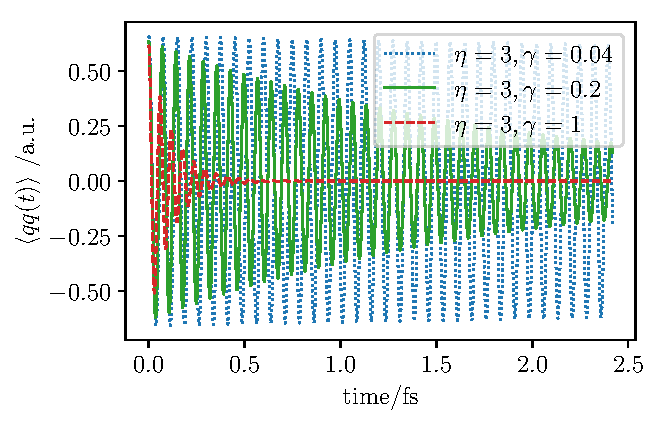
\includegraphics [width=11cm]{qheom_tcf_gamma.pdf}
	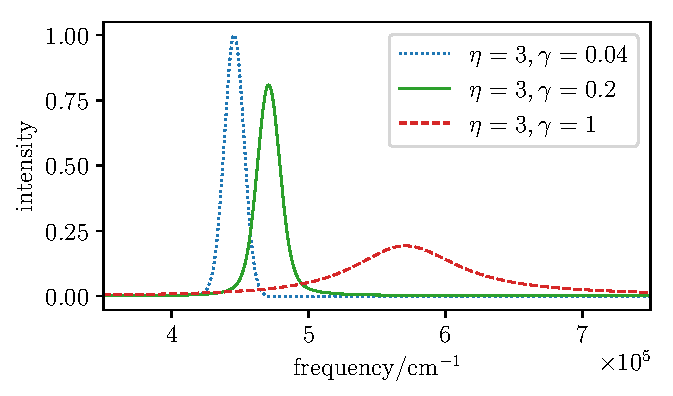
\includegraphics [width=11cm]{qheom_tcf_gamma_spectrum.pdf}
	\caption{
		Position time-autocorrelation function and its spectrum for the harmonic oscillator model system from Tanimura, Wolynes, \emph{Phys.~Rev.~A}, 1991, \textbf{43}, 4131–4142, calculated using high temperature HEOM with truncated Matsubara terms in the bath time autocorrelation function as a function of the bath cutoff frequency $\gamma$ at $\beta=0.4$ a.u.
	}
	\label{fig:qheom_tcf_gamma}
\end{figure}
\begin{figure} [htp!] %pro lepsi obplouvani textu
	\centering
	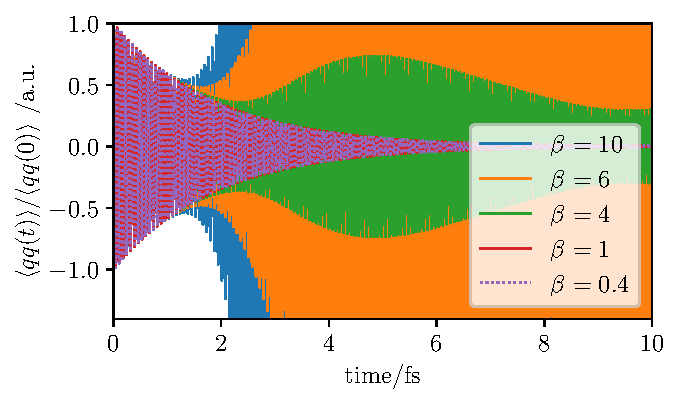
\includegraphics [width=11cm]{qheom_tcf_beta.pdf}
	\caption{
		Normalised position time autocorrelation functions of the harmonic oscillator from fig.~\ref{fig:qheom_tcf_gamma} showing artificial beats when temperature enters the quantum regime ($\beta\hbar\Omega\gg1$). These artefacts are a consequence of the truncation of the Matsubara terms in the bath time autocorrelation function.
	}
	\label{fig:qheom_tcf_beta}
\end{figure}
\newpage

\section{Classical HEOM}\label{sec:cheom}
Similarly to quantum HEOM in section~\ref{sec:qheom}, classical HEOM propagation given by eq.~\ref{eq:cheom} was implemented. Wigner functions were represented in a discretised position-momentum phase space to give
\begin{multline}
\frac{\partial W_{n}(q_i,p_j)}{\partial t}=-\left(\hat{\mathcal{L}}_\mathrm{C} +n \gamma \right)W_{n}(q_i,p_j)\\
+ \frac{\partial W_{n+1}(q_i,p_j)}{\partial p}
+\frac{n\eta\gamma}{\beta} \left(\frac{\partial}{\partial p} - \beta \gamma q\right)W_{n-1}(q_i,p_j).
\end{multline}
To construct the first derivative matrices, an appropriate discrete variable representation (DVR) matrix was derived analogously to the second derivative matrix presented in reference \cite{Colbert1992} to give
\begin{equation}
	D_{ij}=\frac{\pi}{(N+1)L}\times
	\begin{cases}
	Y\left(\frac{(i+j)\pi}{N+1}\right)& \text{for }i=j, \\
	Y\left(\frac{(i+j)\pi}{N+1}\right)
	+Y\left(\frac{(i-j)\pi}{N+1}\right)& \text{otherwise,}
	\end{cases}
\end{equation}
with
\begin{equation}
	Y(x) = \frac{+N\sin\left[(N+1)x\right]-(N+1)\sin(Nx)}{2(1-\cos x)},
\end{equation}
where $N$ is the number of grid points and $L\equiv q_N-q_0$ is the span of the grid.

Similar tests to those described for quantum HEOM in section~\ref{sec:qheom} were carried out. The response to the shifting harmonic oscillator is presented in section~\ref{subsec:cheom_shifting_potential} and calculation of TCFs in section~\ref{subsec:cheom_tcfs}.
\subsection{Shifting potential}\label{subsec:cheom_shifting_potential}
Using the same set-up as described in section~\ref{subsec:qheom_shifting_potential}, a wavepacket was propagated in a shifting potential. Similar studies to those presented for quantum HEOM were carried out and are shown in figures \ref{fig:cheom_contour} and \ref{fig:cheom_position} side by side with the quantum calculations. The trends are the same as before. Increasing bath strength $\eta$ and increasing cutoff frequency $\gamma$ both increase damping. However, the dynamics is different and the classical wave packet oscillates at a higher frequency compared to its quantum counterpart. Upon decreasing the temperature, classical HEOM begins to exhibit a similar divergent behaviour to that of fig.~\ref{fig:qheom_tcf_beta} which leads to poor stability of the calculations.
\begin{figure} [htp!] %pro lepsi obplouvani textu
	\centering
	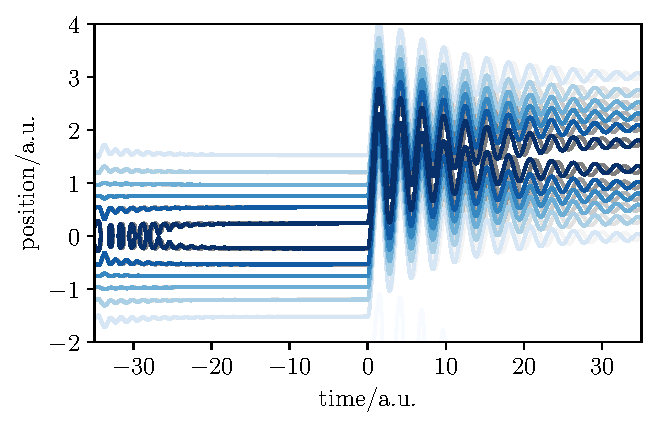
\includegraphics [width=11cm]{cheom_contour.pdf}
	\caption{
		A contour plot of the same shifting potential set-up presented in fig.~\ref{fig:qheom_contour} with classical HEOM in blue and the quantum analogue in grey.
	}
	\label{fig:cheom_contour}
\end{figure}
\begin{figure} [hp!] %pro lepsi obplouvani textu
	\centering
	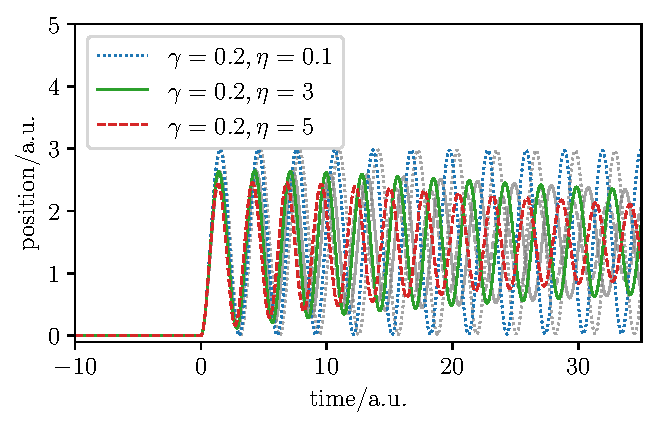
\includegraphics [width=11cm]{comparison_position_eta.pdf}
	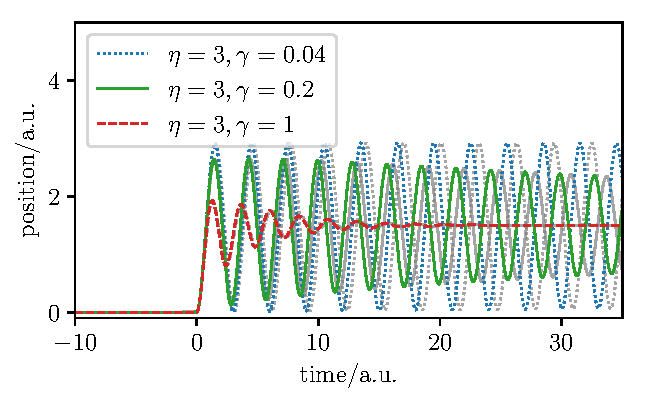
\includegraphics [width=11cm]{comparison_position_gamma.pdf}
	\caption{
		Displacement of the wavepacket centre (average) for a set-up identical to that of fig.~\ref{fig:qheom_position} as a function of the bath strength $\eta$ and the bath cutoff frequency $\gamma$ with classical HEOM in colour and the quantum analogues in grey.
	}
	\label{fig:cheom_position}
\end{figure}
\newpage
\subsection{Harmonic potential TCFs}\label{subsec:cheom_tcfs}
As shown in figure~\ref{fig:cheom_tcf_eta}, the trend of decreasing decorrelation time with increasing bath strength and cutoff frequency is qualitatively the same as for quantum HEOM. Classical HEOM, however, shows a blue shift relative to the quantum result.
\begin{figure} [htp!] %pro lepsi obplouvani textu
	\centering
	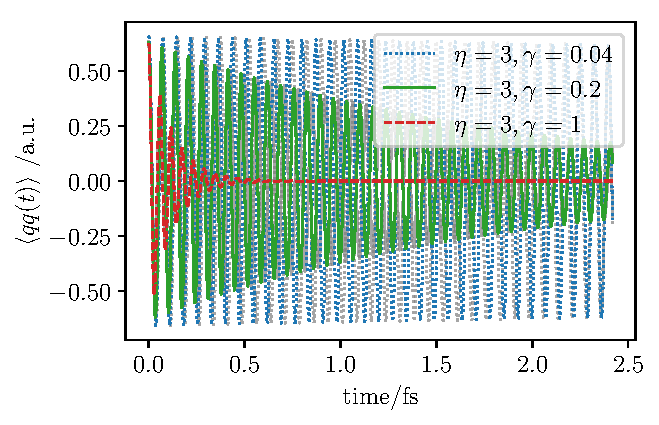
\includegraphics [width=11cm]{comparison_tcf_gamma.pdf}
	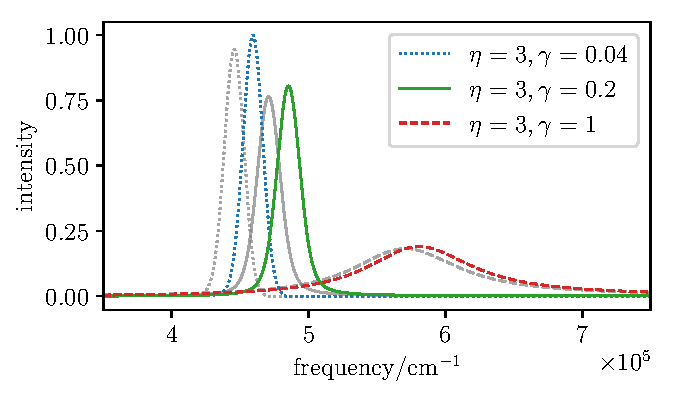
\includegraphics [width=11cm]{comparison_tcf_gamma_spectrum.pdf}
	\caption{
		Position time autocorrelation functions with changing bath cutoff frequency $\gamma$ and their spectra for a set-up identical to fig.~\ref{fig:qheom_tcf_gamma} with classical HEOM in colour and the quantum analogues in grey.
	}
	\label{fig:cheom_tcf_eta}
\end{figure}
\newpage
\section{Low-temperature quantum HEOM}\label{sec:qheom_low_temp}
As shown in section~\ref{sec:qheom}, at low temperatures the Matsubara terms in the bath become necessary for a correct physical description. Therefore, one must use the full quantum HEOM given by equation~\ref{eq:eom_real}. This requires a new computational treatment since ADOs are now spread across a $K+1$ dimensional space. In addition, it is not computationally feasible to represent all ADOs up to a hard cutoff $L$ (i.e.~with tiers $n\le L$) because their number grows combinatorially.\footnote[2]{One can easily show that $N_\mathrm{ADOs}(L,K) = \sum_{n=0}^{L}\binom{n+K}{n}$. (This is an example of the so called ``stars and bars" combinatorics problem.)}

This has been solved by implementing the ADO hierarchy using a Python dictionary in combination with the pruning mechanism described in section~\ref{subsec:L_truncation}. Even then, the number of ADOs is quite large and their interaction more complex, which leads to higher computational requirements. For simulations with static potentials at low temperatures, however, one can transform the HEOM into the space of Hamiltonian eigenvectors (of the system Hamiltonian $\hat{H}_\mathrm{S}$). These were obtained by direct diagonalisation of the DVR Hamiltonian (eq.~\ref{eq:dvr_ham}). This representation leads to much smaller matrices than in the position eigenstate representation and makes calculations more tractable. To improve the rate of equilibration, the initial state for the anharmonic potentials was taken to be the Boltzmann distribution of the DVR energy levels, as opposed to the analytical distribution for the harmonic oscillator (eq.~\ref{eq:ho_init_state}). The exact initial state is, however, irrelevant, assuming that the system is properly equilibrated before the measurement.

In the next section we have shown that the Matsubara terms correct the previous non-physical beating in the TCFs. To test our model on anharmonic potentials we chose two systems from the literature. A Morse oscillator system investigated by Sakurai and Tanimura\supercite{Sakurai2011} is presented in section~\ref{subsec:morse} and a quartic fit of a hydrated oxonium OH bond potential by Yu and Bowman\supercite{Yu2019} in section \ref{subsec:anharmonic}.

\newpage
\subsection{Harmonic potential TCFs}
The importance of Matsubara terms in the bath autocorrelation function $\alpha$ (eq.~\ref{eq:alpha_series}) was demonstrated in figure~\ref{fig:qheom_tcf_beta}, where lowering the temperature lead to beating or even divergence of the TCF. As figure~\ref{fig:qheom_tcf_low_temp} demonstrates, at $\beta=10$~a.u., which is deep in the ``quantum regime"($\beta\hbar\Omega= 20 \gg1$), two Matsubara terms are already qualitatively correct, with $K=3$ yielding the converged result. The number of Matsubara modes required increases with decreasing temperature as expected, since more terms in the exponential series of $\alpha$ will contribute.
\begin{figure} [htp!] %pro lepsi obplouvani textu
	\centering
	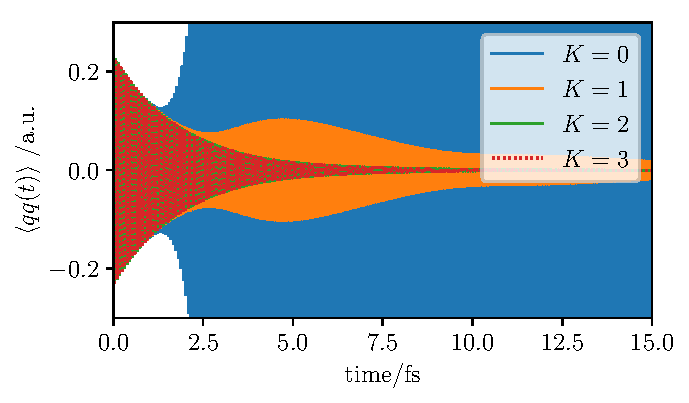
\includegraphics [width=11cm]{qheom_tcf_low_temp.pdf}
	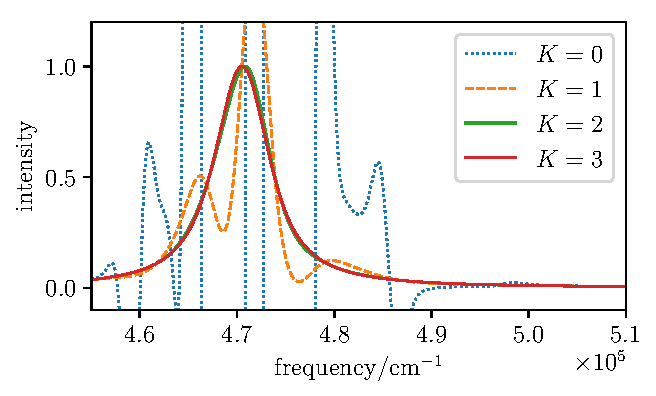
\includegraphics [width=11cm]{qheom_tcf_low_temp_spectrum.pdf}
	\caption{
		Low temperature correction to a TCF from figure~\ref{fig:qheom_tcf_beta} at $\beta=10\mathrm{\ a.u.}$ and its spectrum. It can be seen that at this temperature inclusion of two Matsubara terms already leads to an almost converged result and three are sufficient. Decreasing temperature leads to an increase in the number of required Matsubara terms in the bath autocorrelation function.
	}
	\label{fig:qheom_tcf_low_temp}
\end{figure}
\newpage
\subsection{Morse potential TCFs} \label{subsec:morse}
Tanimura and Sakurai have studied HEOM spectra for the Morse potential,\supercite{Sakurai2011} which is defined as
\begin{equation}
	V_\mathrm{Morse}(q) = D_\mathrm{e}\left(1-\mathrm{e}^{-\alpha q}\right)^2 ,
\end{equation}
where $D_\mathrm{e}$ is the depth of the potential well and $\alpha$ is the stiffness coefficient. They chose the values $\Omega_{10} = 1600\mathrm{\ cm^{-1}}$ and $\Delta_\mathrm{anh} = 16\mathrm{\ cm^{-1}}$ which are related to potential parameters as  $\Delta_\mathrm{anh} = \hbar\alpha^2/m$ and $\Omega_\mathrm{c} = \sqrt{2 D_\mathrm{e}\alpha^2/m}$ with $\Omega_{10} = \Omega_\mathrm{c} - \Delta_\mathrm{anh}$. The authors relate these values to the Amide-I mode in peptides.

Calculations were carried out at the temperature of 300 K at which quantum effects are pronounced, with a bath strength $\eta = 0.05\Omega_{10}$, and with varying bath cutoff frequency $\gamma = 0.02\Omega_{10}$, $0.1\Omega_{10}$ and $0.5\Omega_{10}$. Sakurai and Tanimura's results are compared with our results in figure \ref{fig:morse}. The positions and shapes of peaks in our quantum HEOM spectra follow the published results closely, including a minor feature of the 1--2 transition at $\sim$1585 $\mathrm{cm^{-1}}$. Despite our calculations being converged with respect to all parameters, the observed magnitude of this transition for the $\gamma = 0.02\Omega_{10}$ case was smaller than the reported value. The origin of this discrepancy is currently unknown.

As opposed to Sakurai's calculations which used a rigid cutoff in $L$ with an anchor equation, in our simulation we settled with scaling and pruning due to Shi as described in section~\ref{subsec:L_truncation}. This allows the number of ADOs to dynamically change during the simulation. Results have been converged both with respect to the number of Matsubara terms $K$ and the pruning cutoff (equivalent to converging w.r.t.~$L$). It was found that inclusion of the low temperature correction due to Tanimura (eq.~\ref{eq:low_temp_correction}) improves the $K$\=/convergence greatly. This effect is particularly pronounced during equilibration, where the drift of the wave packets described in section~\ref{subsec:qheom_tcfs} shows relatively slow convergence without the correction.
\begin{figure} [htp!] %pro lepsi obplouvani textu
	\centering
	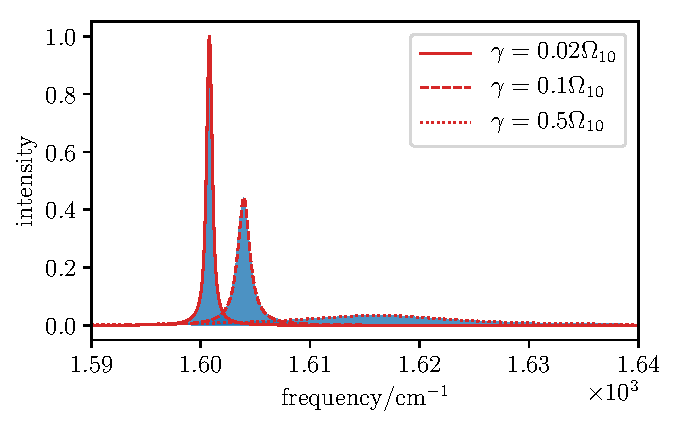
\includegraphics [width=11cm]{morse_2000_corr_spectrum.pdf}
	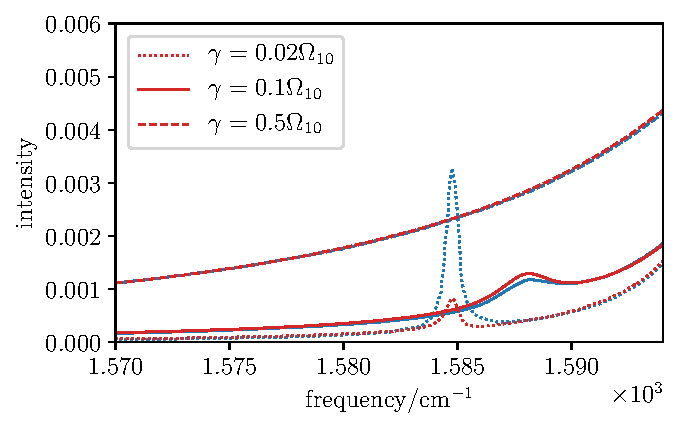
\includegraphics [width=11cm]{morse_2000_corr_spectrum_spectrum_inset.pdf}
	\caption{
		Morse oscillator quantum HEOM spectra at 300 K with varying bath cutoff frequency $\gamma$ and a magnification of the 1--2 transition. The shaded areas in the first graph and the blue lines in the second are the results extracted from Sakurai, Tanimura, \emph{J.~Phys.~Chem.~A}, 2011, \textbf{115}, 4009-4022.
	}
	\label{fig:morse}
\end{figure}
\newpage
\subsection{Anharmonic OH model TCFs} \label{subsec:anharmonic}
Yu and Bowman have recently published their calculation of water cluster vibrational spectra.\supercite{Yu2019} Most commonly used quantum dynamics methods, including thermostatted ring-polymer
molecular dynamics (TRPMD), perform poorly in these strongly anharmonic potentials.\supercite{Yu2019}

Raz Benson investigated this behaviour, by fitting the $\mathrm{H_7O_3^+}$ OH potential used by Bowman with a quartic polynomial, and calculating its white-noise TRPMD TCFs. The form of the potential is
\begin{equation}
	V_\mathrm{S} [\mathrm{a.u.}]= 0.1297 q^2 + c (0.1657 q^4 - 0.2467 q^3),
\end{equation}
where $c$ is the anharmonicity coefficient, which for $c=1$ gives a quartic fit to the original potential. The temperature was set to 100 K and the effective mass used is $m = 1837.3622\mathrm{\ a.u.}$

Benson's preliminary results show a large blue shift relative to exact quantum results as shown in figure~\ref{fig:raz_data}.\footnote[2]{Exact quantum results were obtained using discrete variable representation (DVR)\supercite{Colbert1992} Hamiltonian and expansion of eq.~\ref{eq:tcf_qq} in energy eigenstates.} Because we are
particularly interested in the blue shift, we decided to set $a_\mathrm{ren}=0$ in our HEOM calculations. Otherwise, the renormalisation potential in eq.~\ref{eq:renorm_pot} would lead to a blue shift simply by increasing the effective spring constant of the potential. In other terms, we used the convention, in which the renormalisation potential is taken to be a part of the system potential. Other parameters were set to $\eta = 5$ and $\gamma = 0.1\Omega_\mathrm{h}$, where $\Omega_\mathrm{h}$ is the frequency for the harmonic case ($c=0$). The bath strength was chosen such that damping is substantial on the time scale of $\sim$500 fs, which is a typical decorrelation time for liquid water.\supercite{Woutersen1999}

One hypothesis on the possible sources of the TRPMD blue shift relative to DVR is the lack of quantum coherence in PIMD\=/based methods.  HEOM not coupled to the bath ($\eta=0$) gives results identical to DVR and one of the effects of coupling a system to a bath is loss of coherence. If this were a major contributor to the blue shift, we would expect to see HEOM shifted to higher frequencies relative to DVR. However, it was observed that under the previously described set-up, inclusion of a bath results in a small red shift relative to DVR as shown in fig.~\ref{fig:raz_comparison}. It is not clear at this stage which effects are simply mechanical and which might be due to loss of coherence, but the collected data does not support the presented hypothesis.

\begin{figure} [htp!] %pro lepsi obplouvani textu
	\centering
	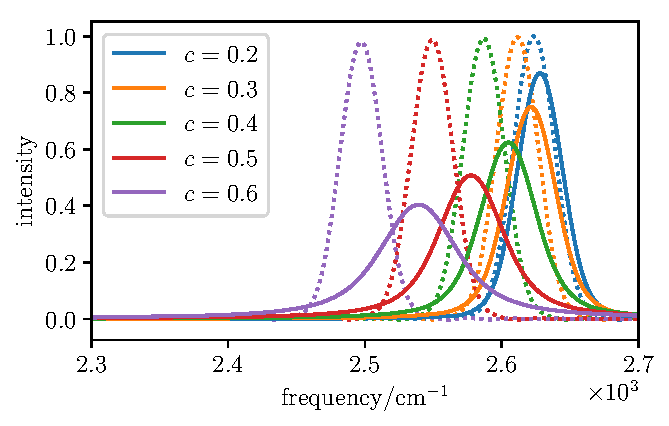
\includegraphics [width=11cm]{raz_spectrum.pdf}
	\caption{
		Benson's white-noise TRPMD spectra for a quartic fit to a hydrated oxonium ion OH potential compared with exact quantum DVR calculations. The coefficient $c$ defines the level of anharmonicity of the potential with $c=0$ being completely harmonic. TRPMD data are shown in full lines and DVR in dotted lines.
	}
	\label{fig:raz_data}
\end{figure}

\begin{figure} [htp!] %pro lepsi obplouvani textu
	\centering
	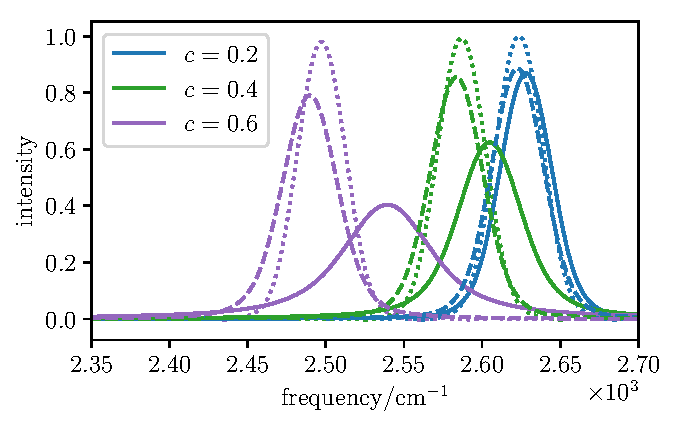
\includegraphics [width=11cm]{raz_comparison_spectrum.pdf}
	\caption{
		Comparison of HEOM spectra for non-renormalised potential with DVR and TRPMD data from figure \ref{fig:raz_data}. TRPMD is shown in full lines, DVR in dotted lines and HEOM in dashed lines. Data for $c=0.3$ and 0.5 were omitted for clarity, but they show the same trend.
	}
	\label{fig:raz_comparison}
\end{figure}

